% !TEX root = ../main.tex
\chapter{Capturas de la Interfaz Web}
\label{anexo:dashboard}

Este apéndice recoge capturas de las seis vistas del cuadro de mandos, organizadas por los dos planos funcionales de la interfaz: el \textbf{plano de Operación} y el \textbf{plano de Análisis}. Se han tomado sobre una instancia local que ejecuta los mismos artefactos que la desplegada, cuya topología describe la Sección~\ref{sec:calidad_despliegue}, leyendo la corrida \texttt{tfg\_latent\_20260831\_113339} del almacén. El selector de la cabecera, presente en todas las vistas, es el que fija esa corrida.

% ─────────────────────────────────────────────
\section*{Plano de Operación}
% ─────────────────────────────────────────────

\begin{figure}[H]
    \centering
    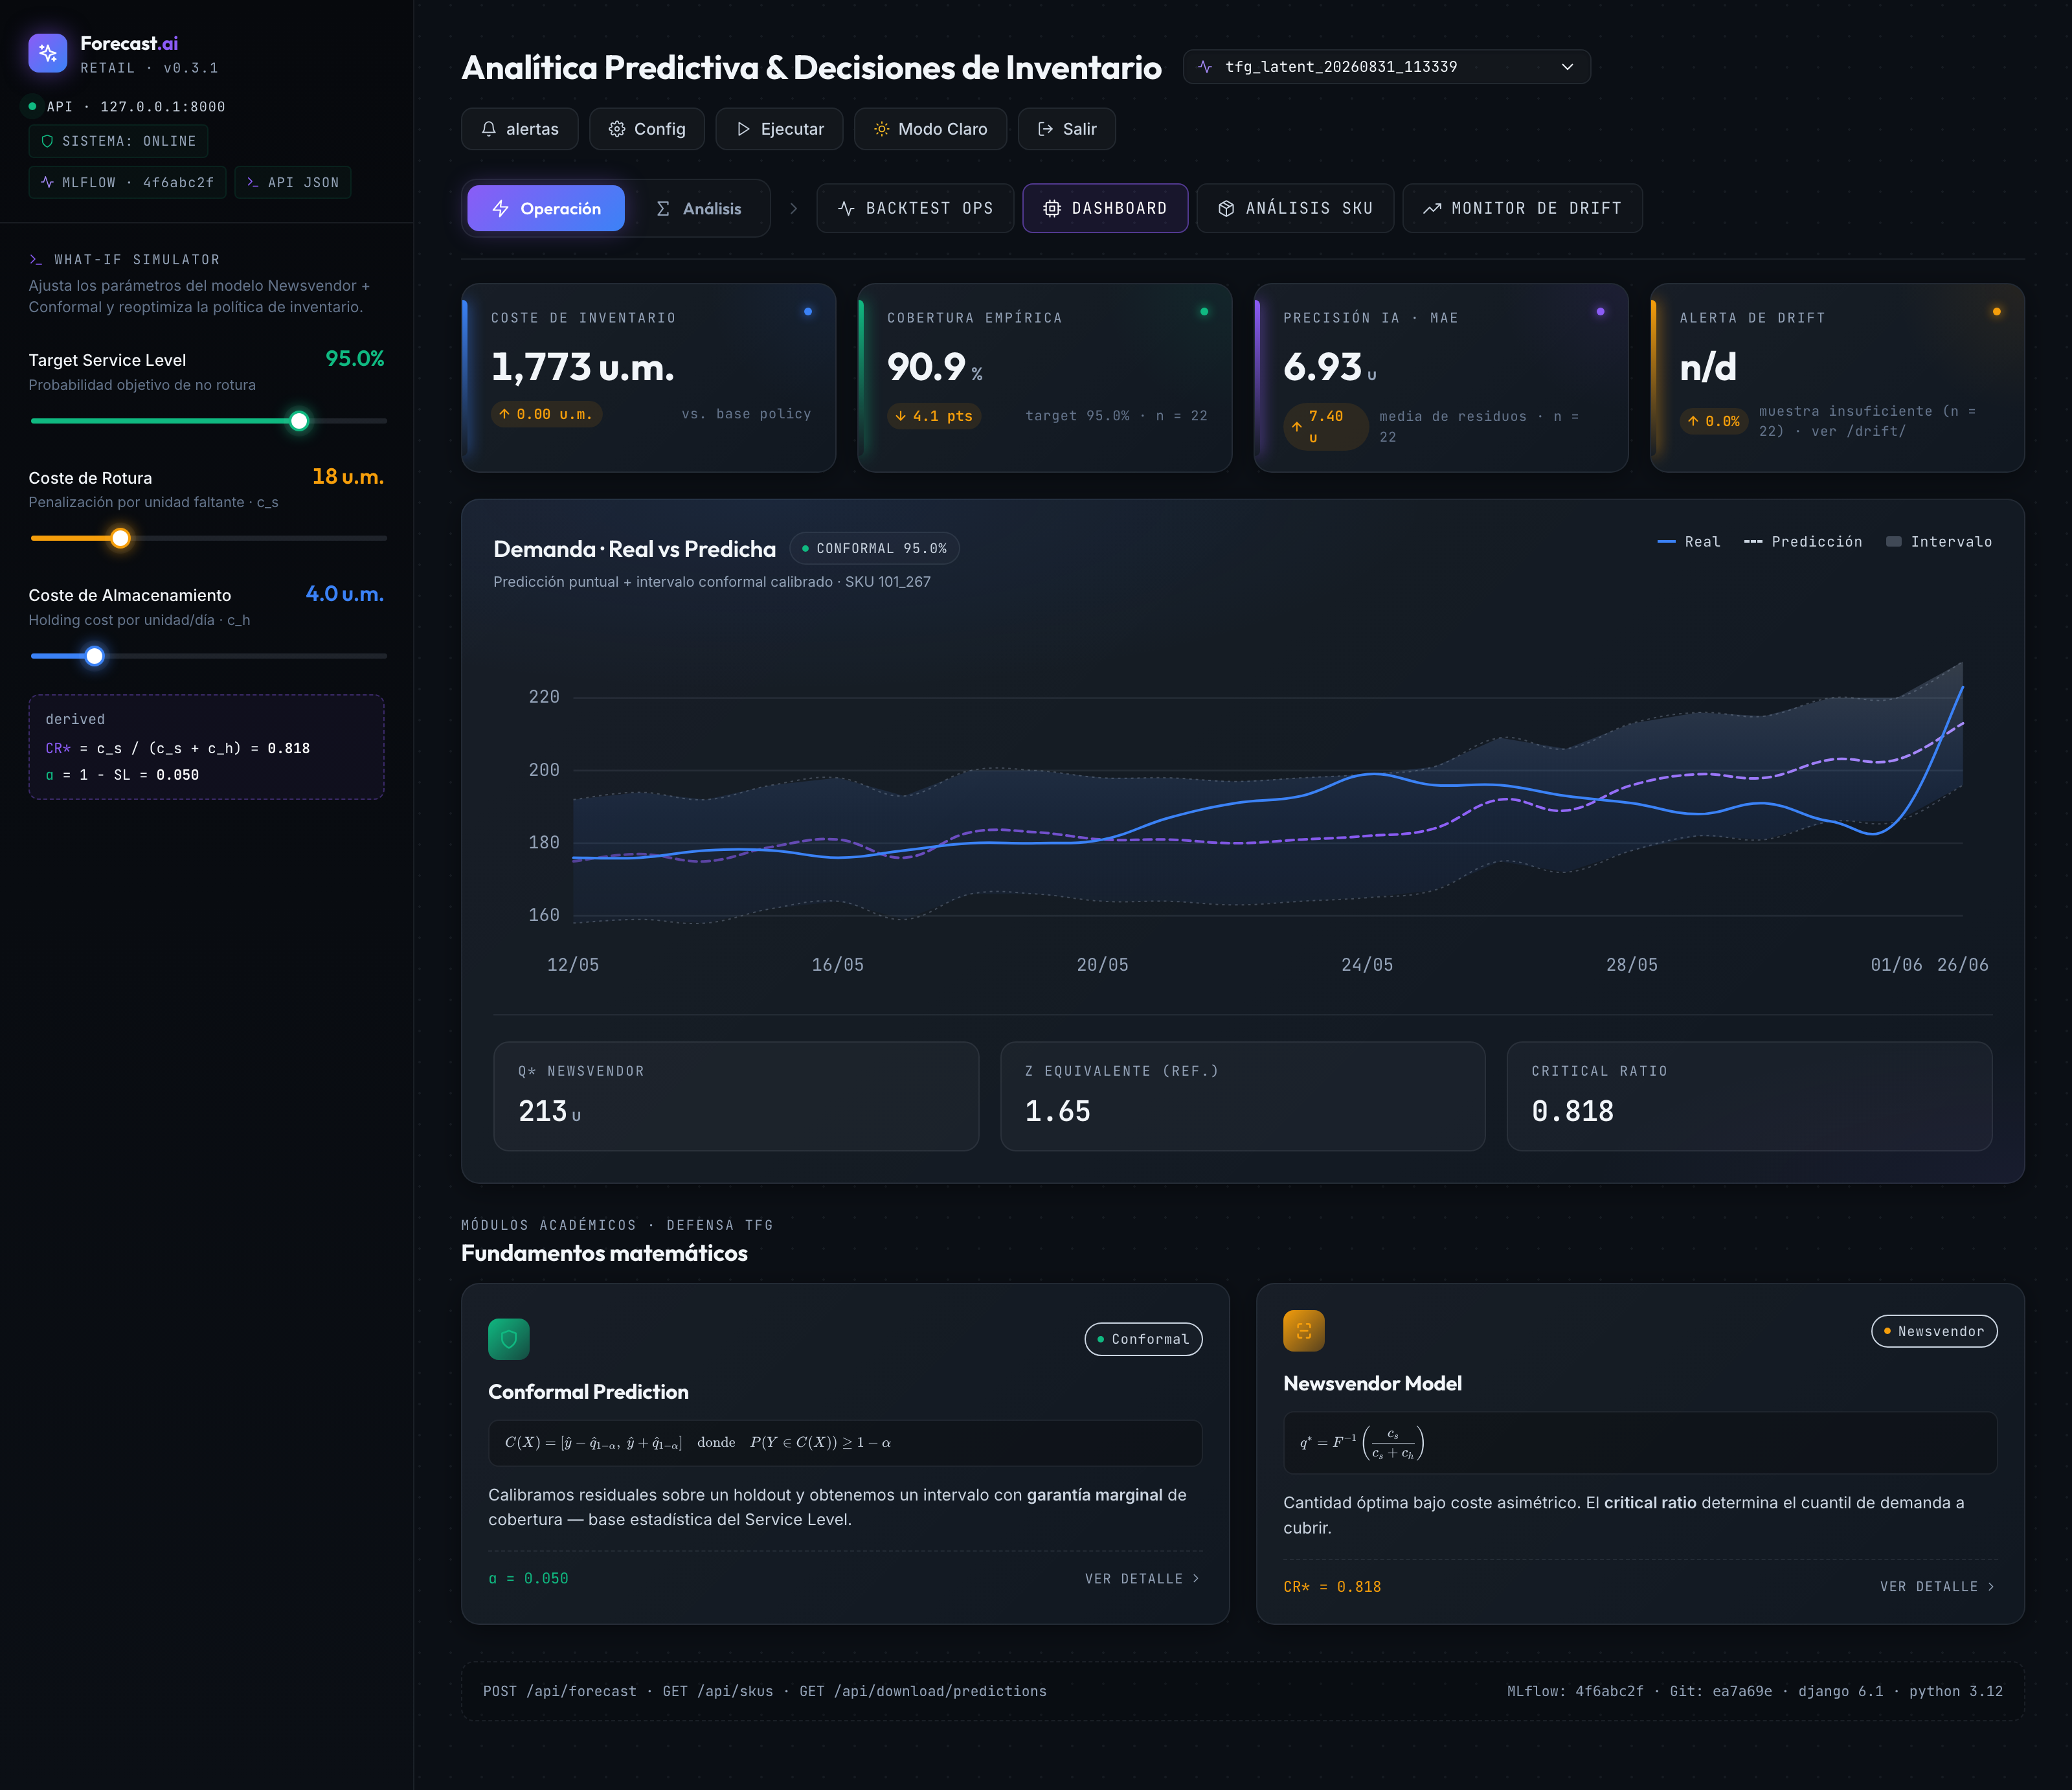
\includegraphics[width=\textwidth,height=0.82\textheight,keepaspectratio]{figures/dashboard/ui_operacion_dashboard.png}
    \caption{Vista \textit{Dashboard} del plano de Operación. Muestra los cuatro KPIs principales (coste de inventario, cobertura empírica, MAE y alerta de drift), el gráfico de demanda real vs. predicha con banda conformal calibrada al 95\,\%, y el simulador \textit{What-If} en el panel lateral izquierdo.}
    \label{fig:ui_operacion_dashboard}
\end{figure}

\begin{figure}[H]
    \centering
    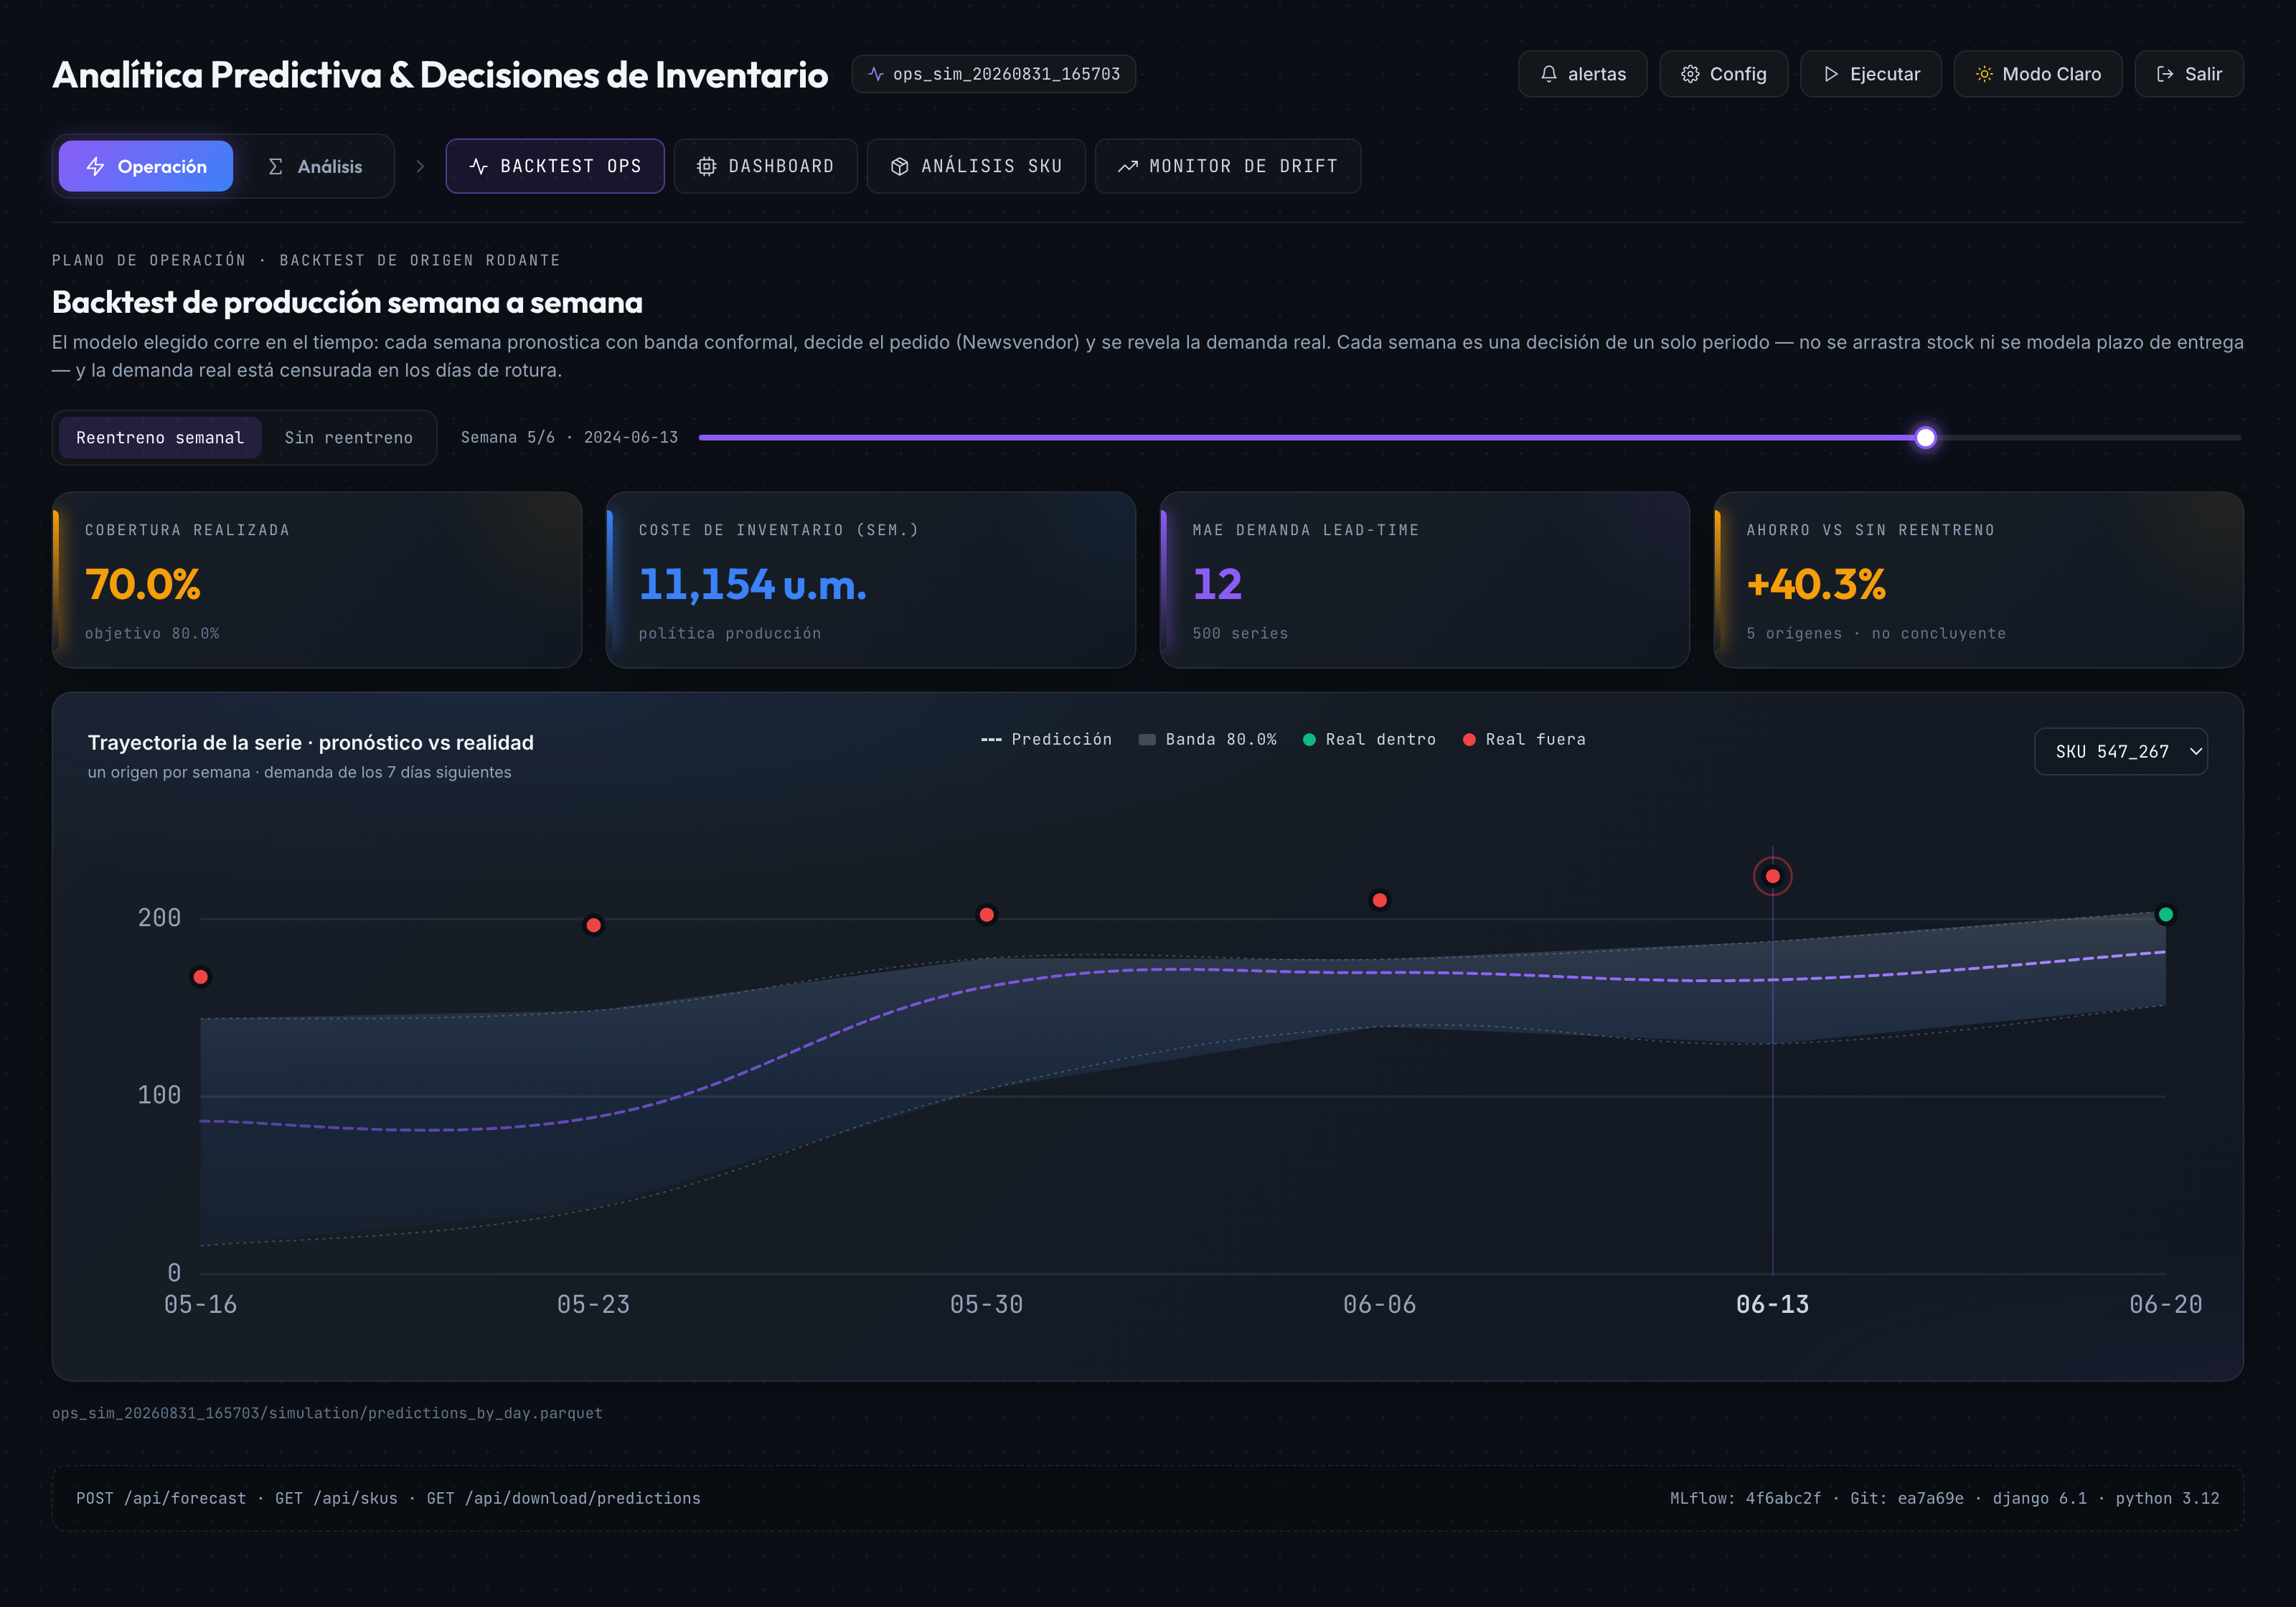
\includegraphics[width=\textwidth,height=0.82\textheight,keepaspectratio]{figures/dashboard/ui_simulacion_ops.png}
    \caption{Vista \textit{Backtest OPS} del plano de Operación. Presenta el backtest de origen rodante semana a semana: cobertura realizada, coste de inventario semanal, MAE de la demanda a \textit{lead time} y ahorro frente a no reentrenar, este último acompañado del número de orígenes que lo sostienen. El conmutador elige entre la política con reentreno semanal y la que mantiene el modelo fijo, y el deslizador recorre las semanas del horizonte evaluado.}
    \label{fig:ui_simulacion_ops}
\end{figure}

\begin{figure}[H]
    \centering
    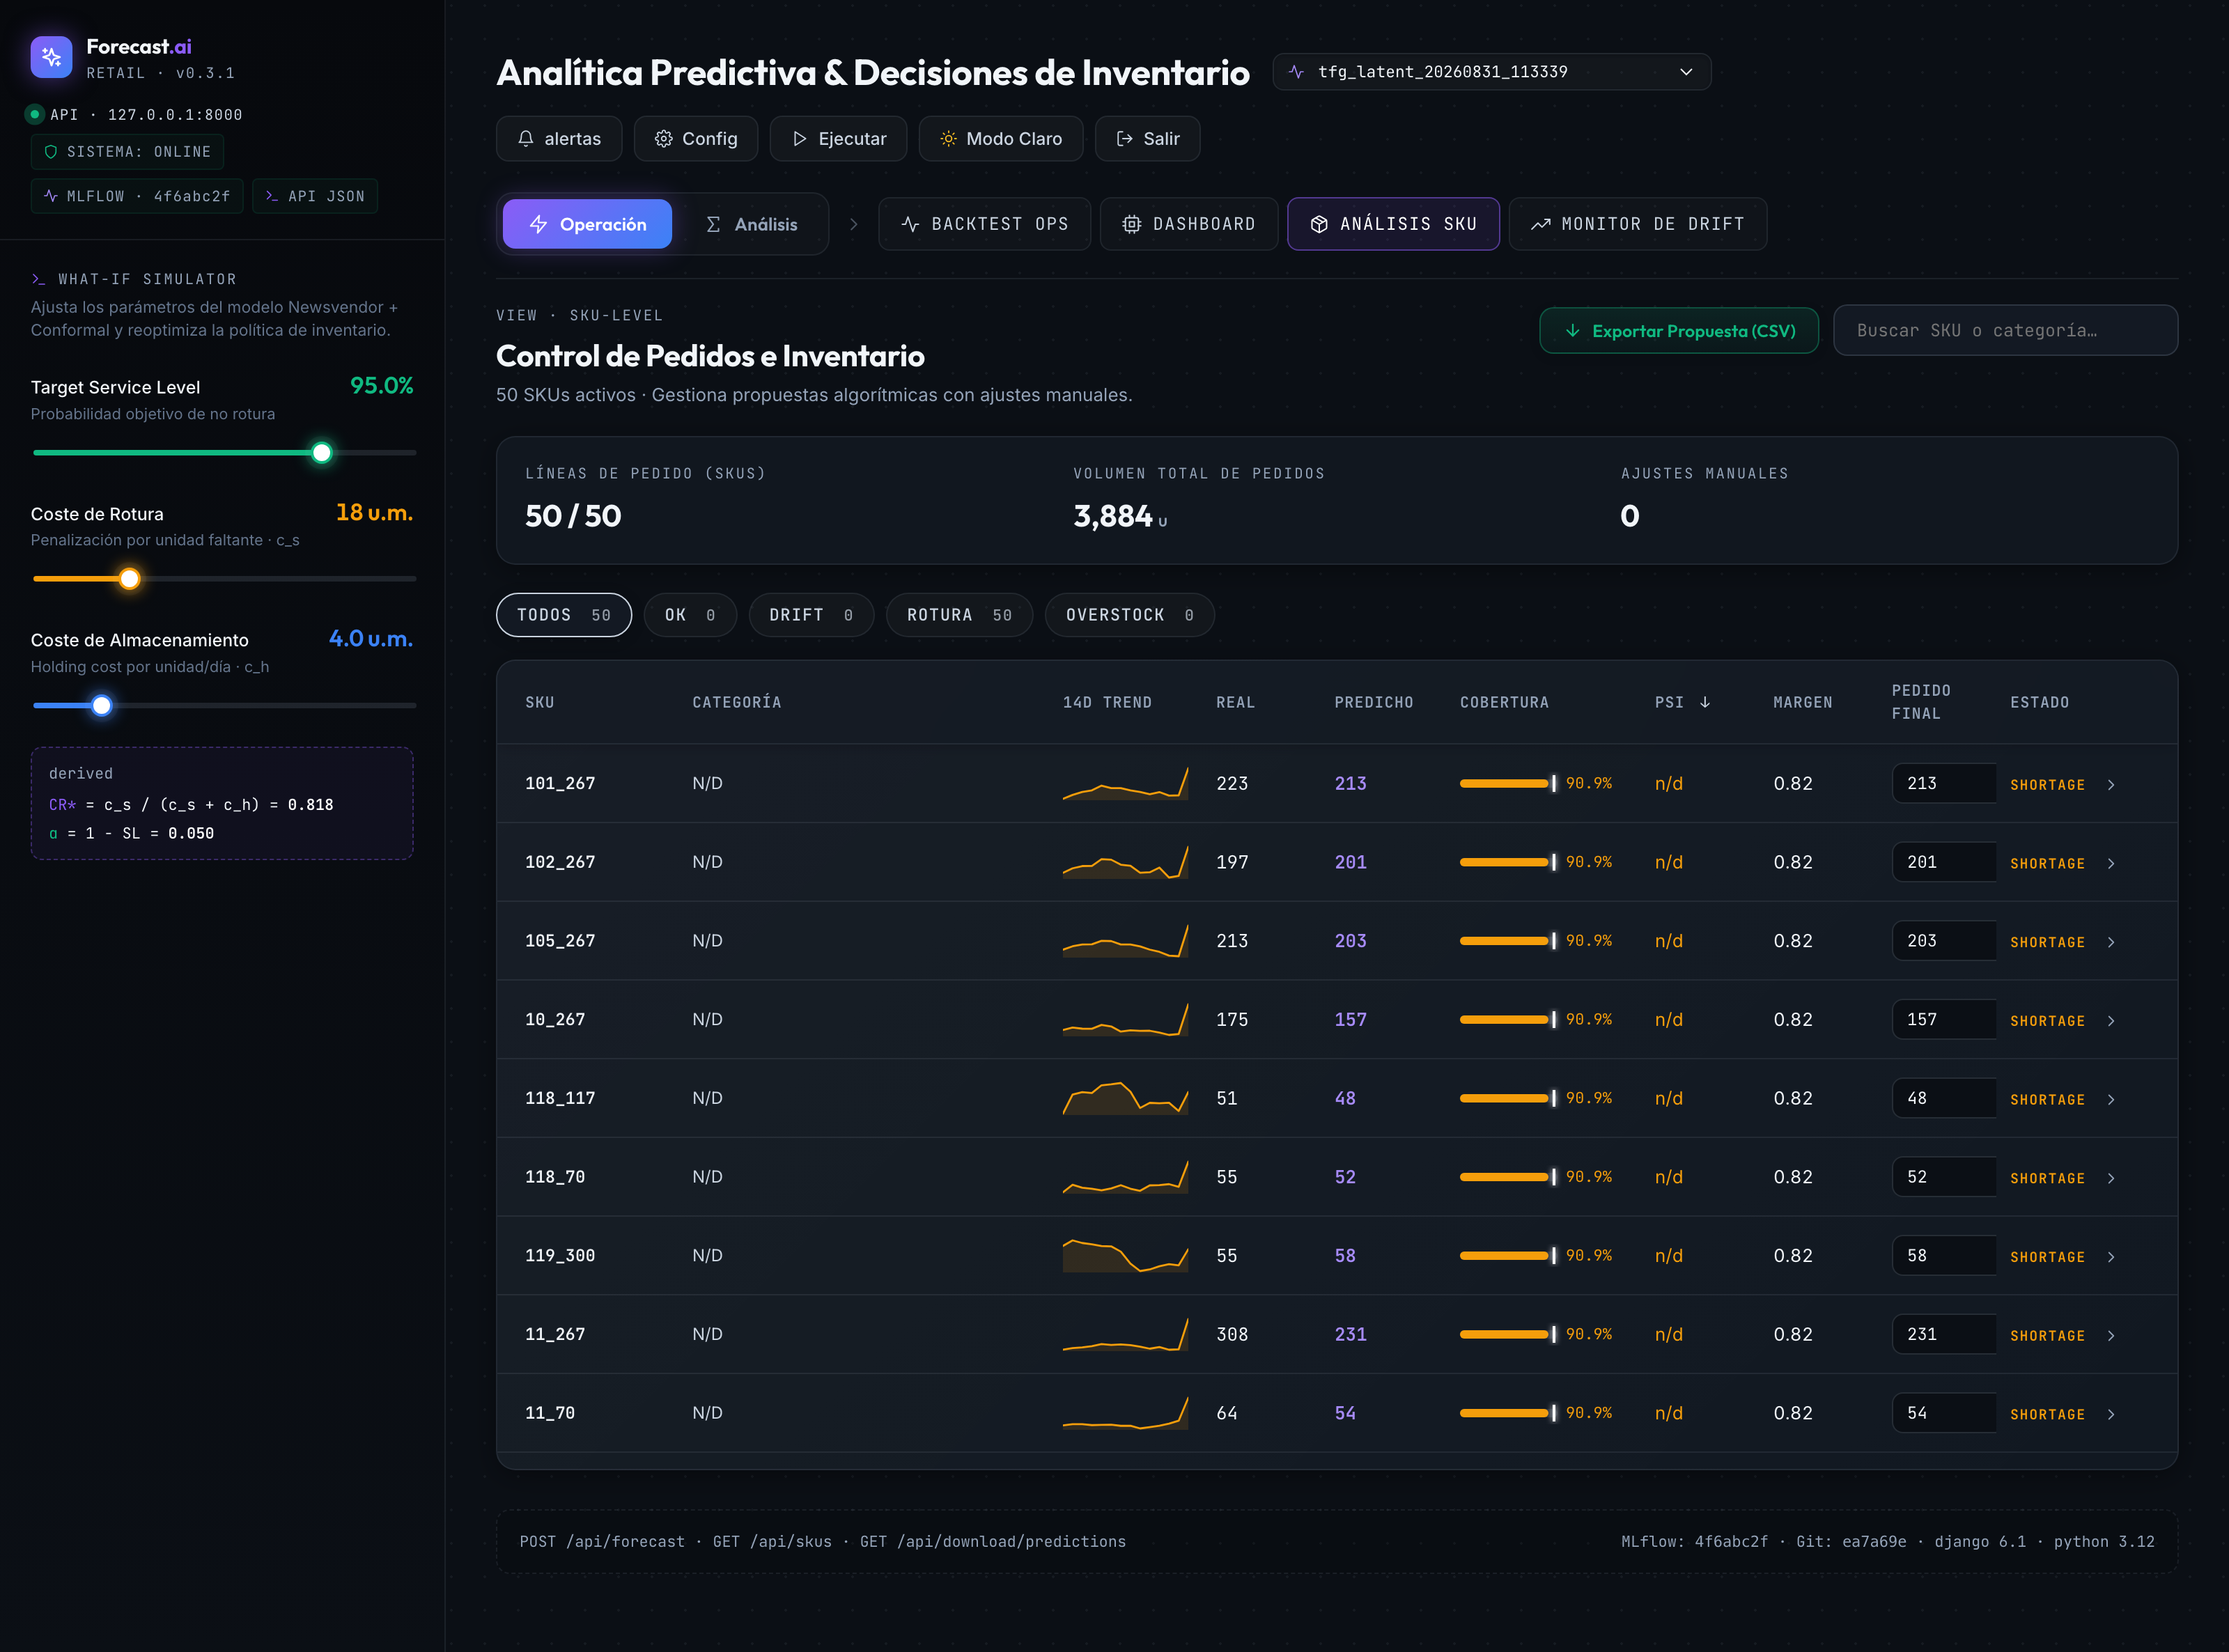
\includegraphics[width=\textwidth,height=0.82\textheight,keepaspectratio]{figures/dashboard/ui_analisis_sku.png}
    \caption{Vista \textit{Análisis SKU} del plano de Operación. Tabla de los 50 SKUs activos con \textit{sparklines} de tendencia de 14 días, cobertura empírica, PSI de drift, pedido propuesto y estado operacional (OK / DRIFT / ROTURA / OVERSTOCK).}
    \label{fig:ui_analisis_sku}
\end{figure}

\begin{figure}[H]
    \centering
    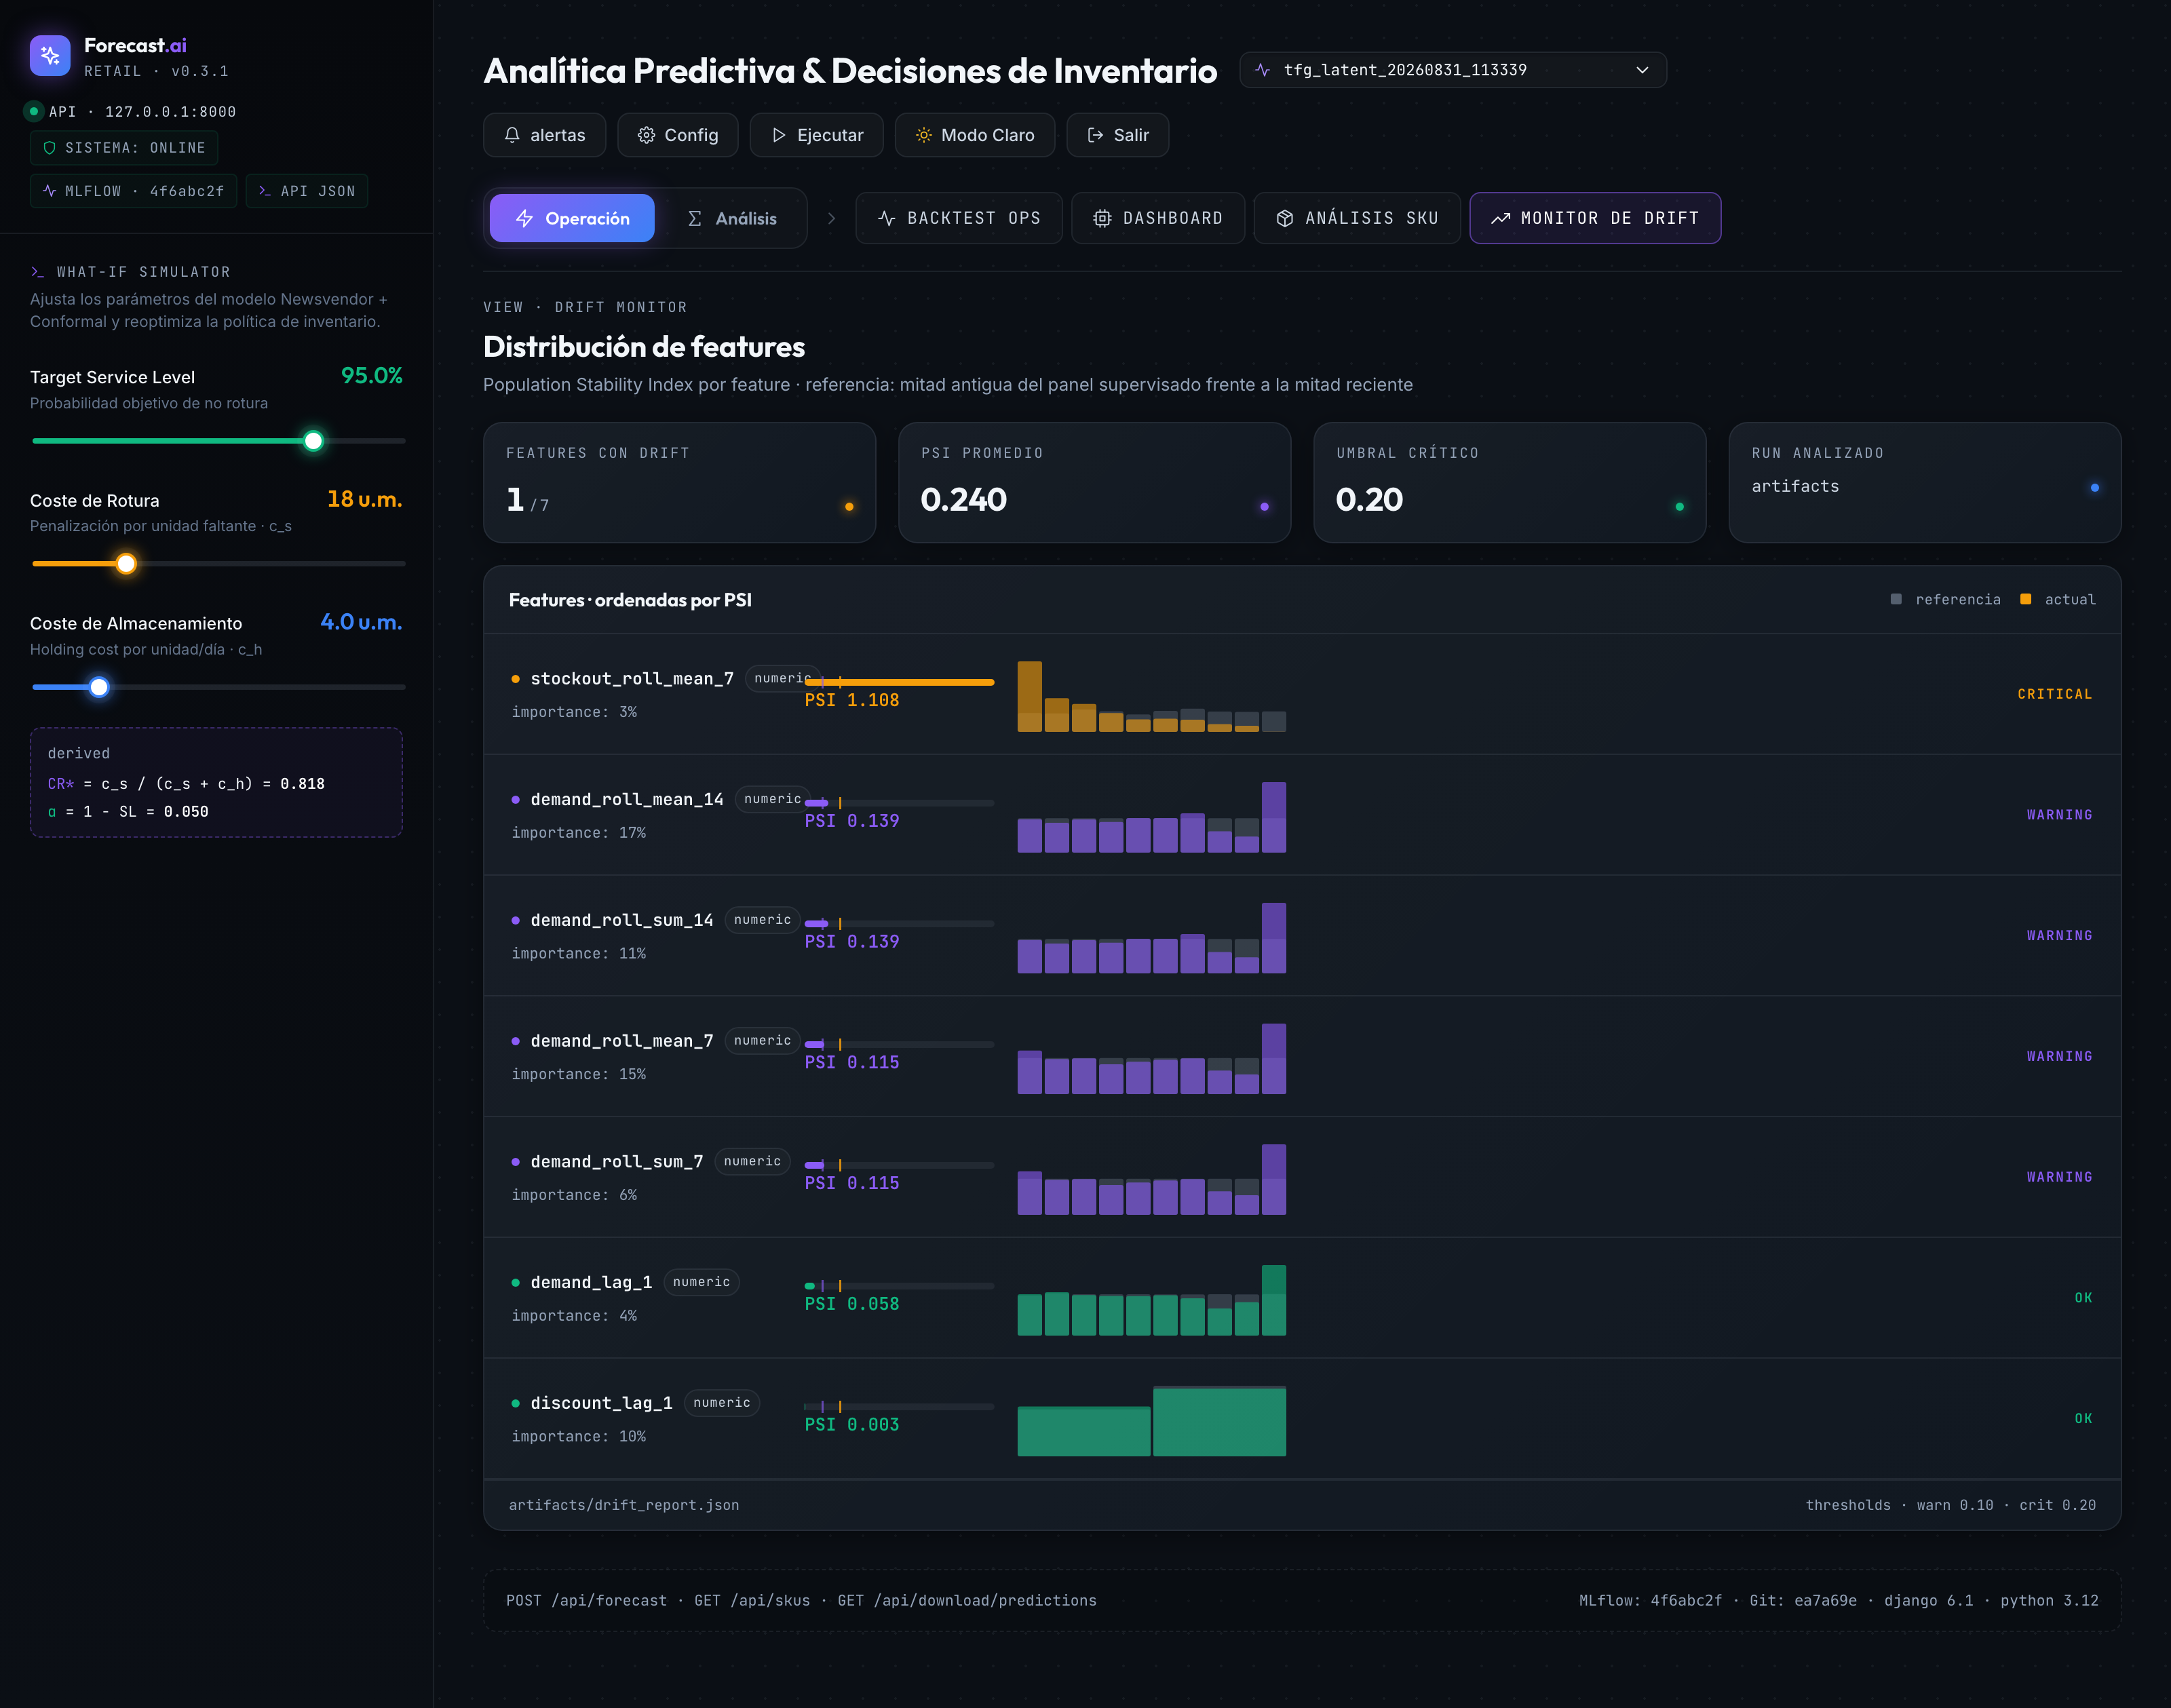
\includegraphics[width=\textwidth,height=0.82\textheight,keepaspectratio]{figures/dashboard/ui_monitor_drift.png}
    \caption{Vista \textit{Monitor de Drift} del plano de Operación. Muestra el PSI de cada feature ordenado de mayor a menor, con umbrales de advertencia (0,10) y crítico (0,20). La cabecera resume el número de \textit{features} con deriva crítica, el PSI promedio, el umbral crítico y la ejecución analizada.}
    \label{fig:ui_monitor_drift}
\end{figure}

% ─────────────────────────────────────────────
\section*{Plano de Análisis}
% ─────────────────────────────────────────────

\begin{figure}[H]
    \centering
    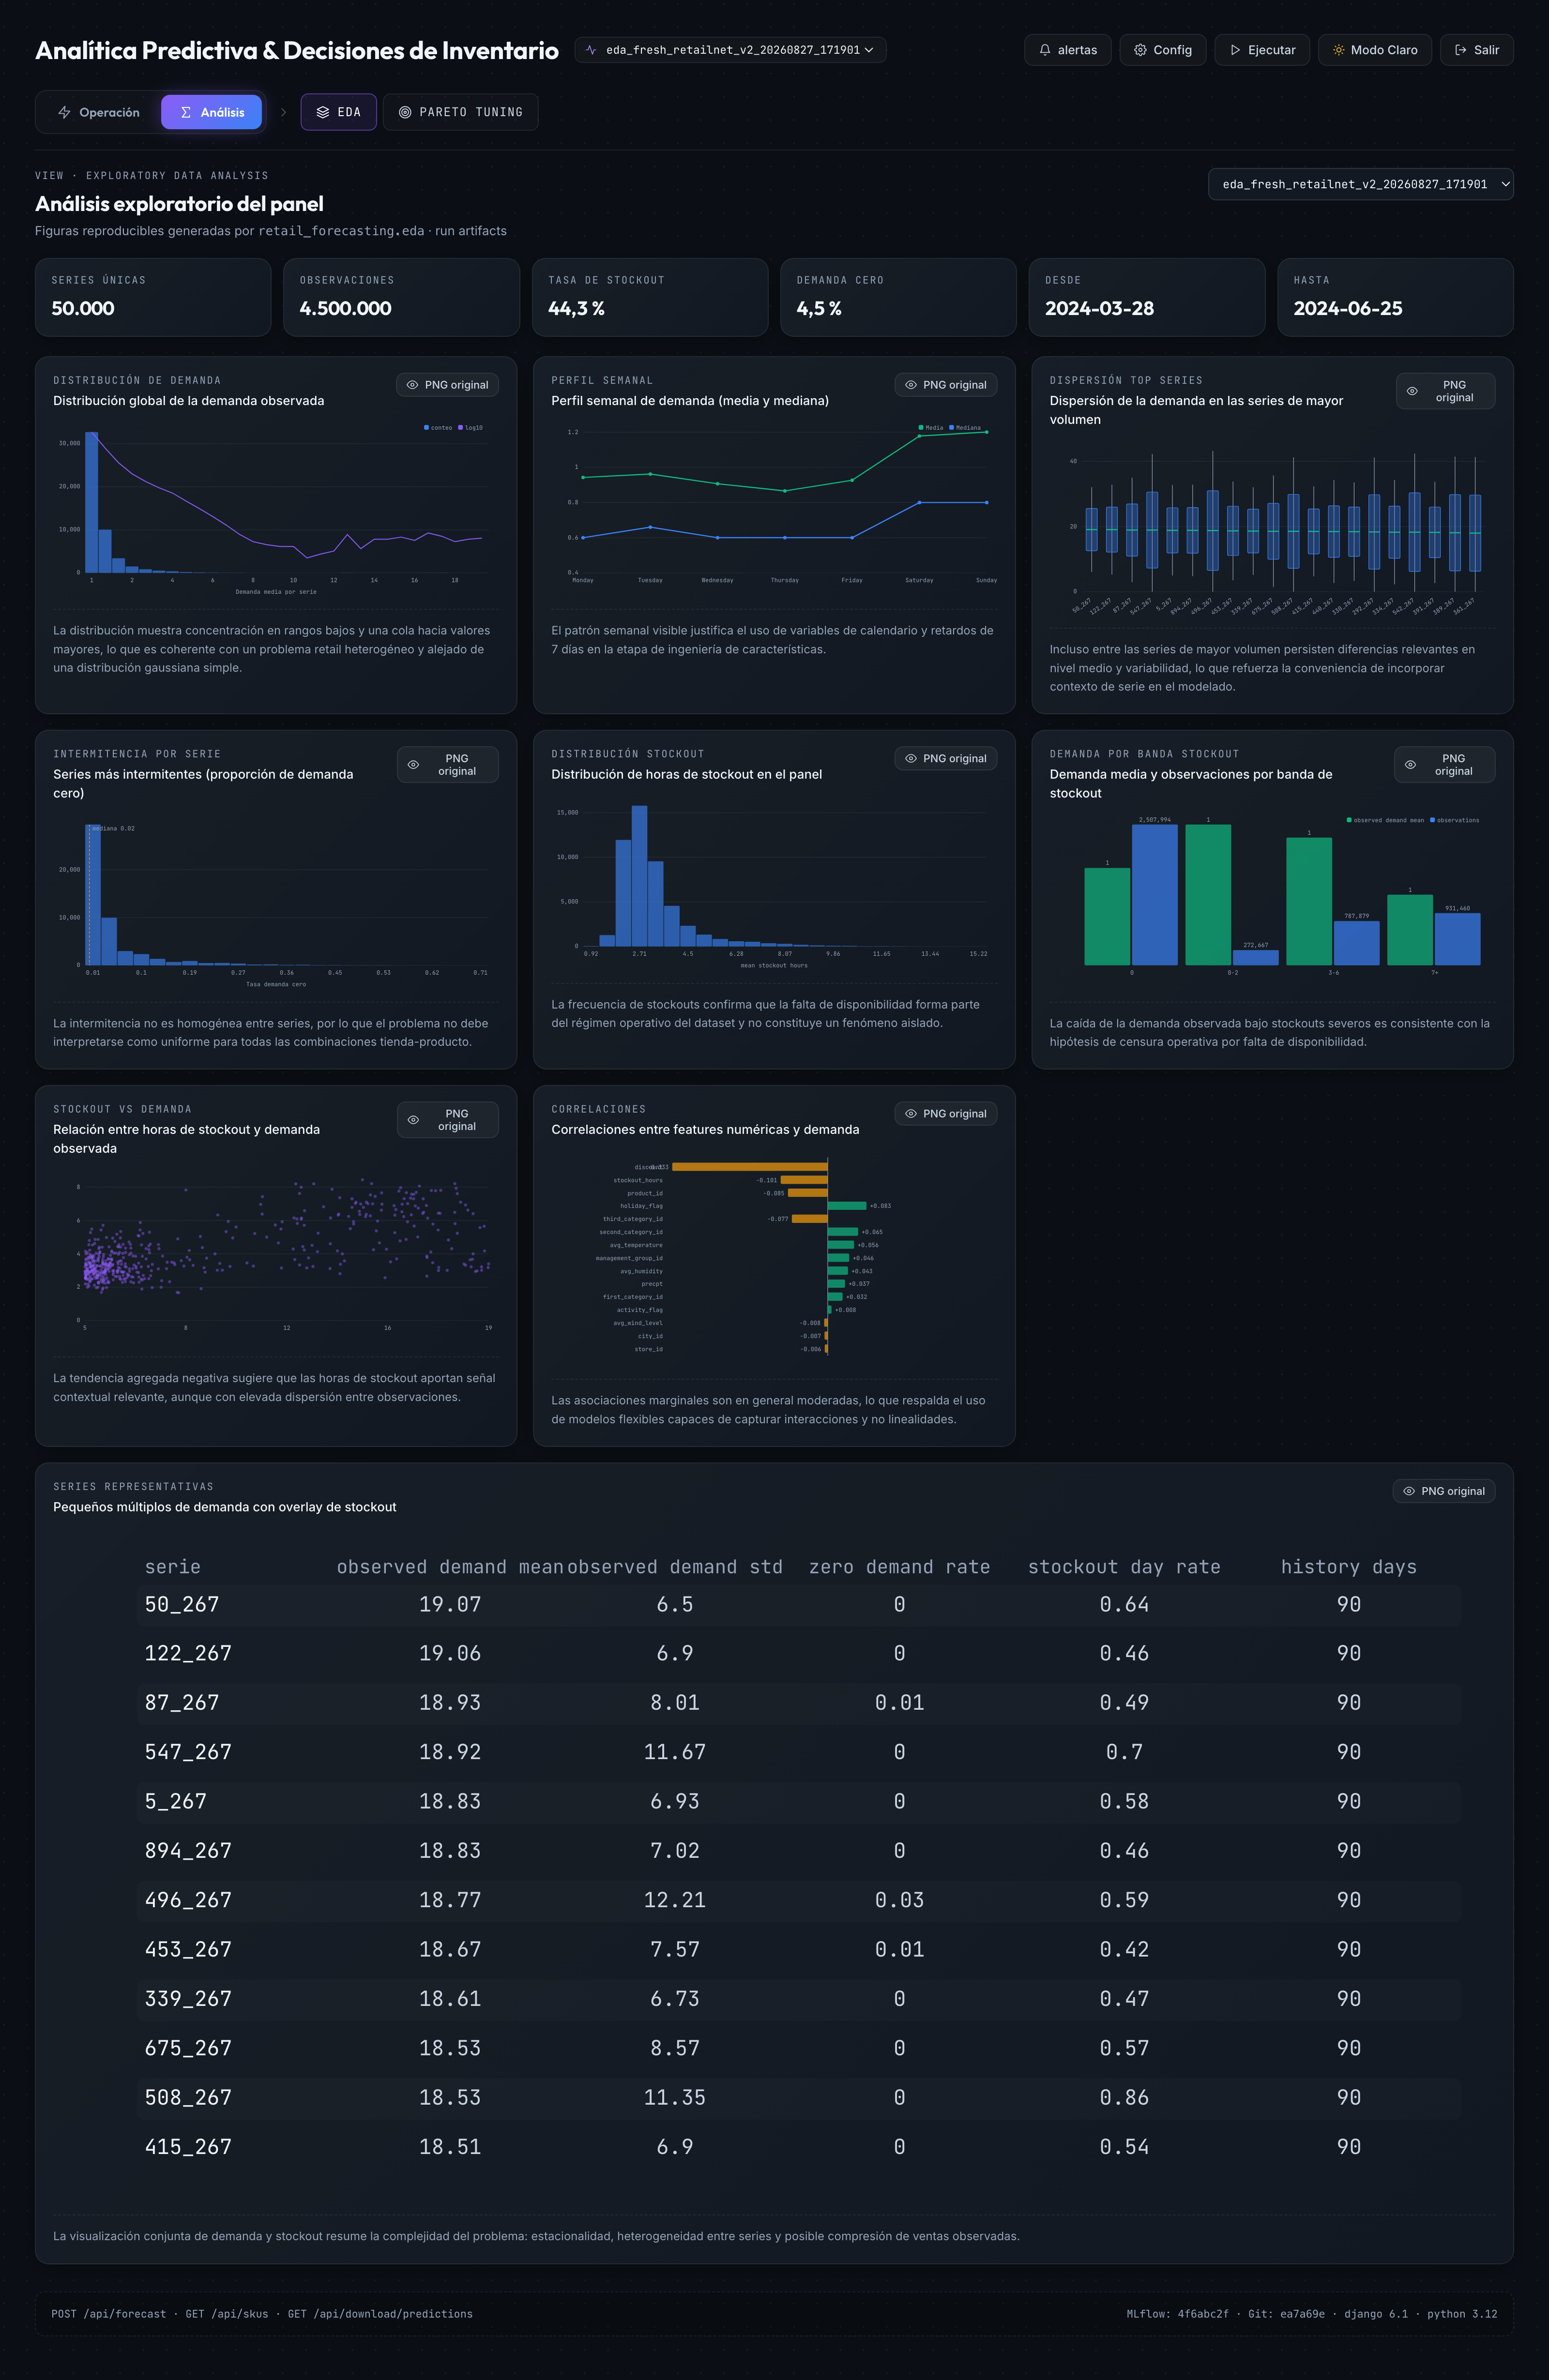
\includegraphics[width=\textwidth,height=0.82\textheight,keepaspectratio]{figures/dashboard/ui_eda_overview.png}
    \caption{Vista \textit{EDA} del plano de Análisis. Panel resumen con estadísticos globales del dataset (50.000 series únicas, 4,5\,M filas, tasa de stockout 44,3\,\%) y las nueve figuras exploratorias, redibujadas como SVG en servidor a partir de los CSV que produce el módulo de análisis exploratorio. Cada figura conserva su interpretación escrita y un enlace al PNG original a resolución completa.}
    \label{fig:ui_eda_overview}
\end{figure}


\begin{figure}[H]
    \centering
    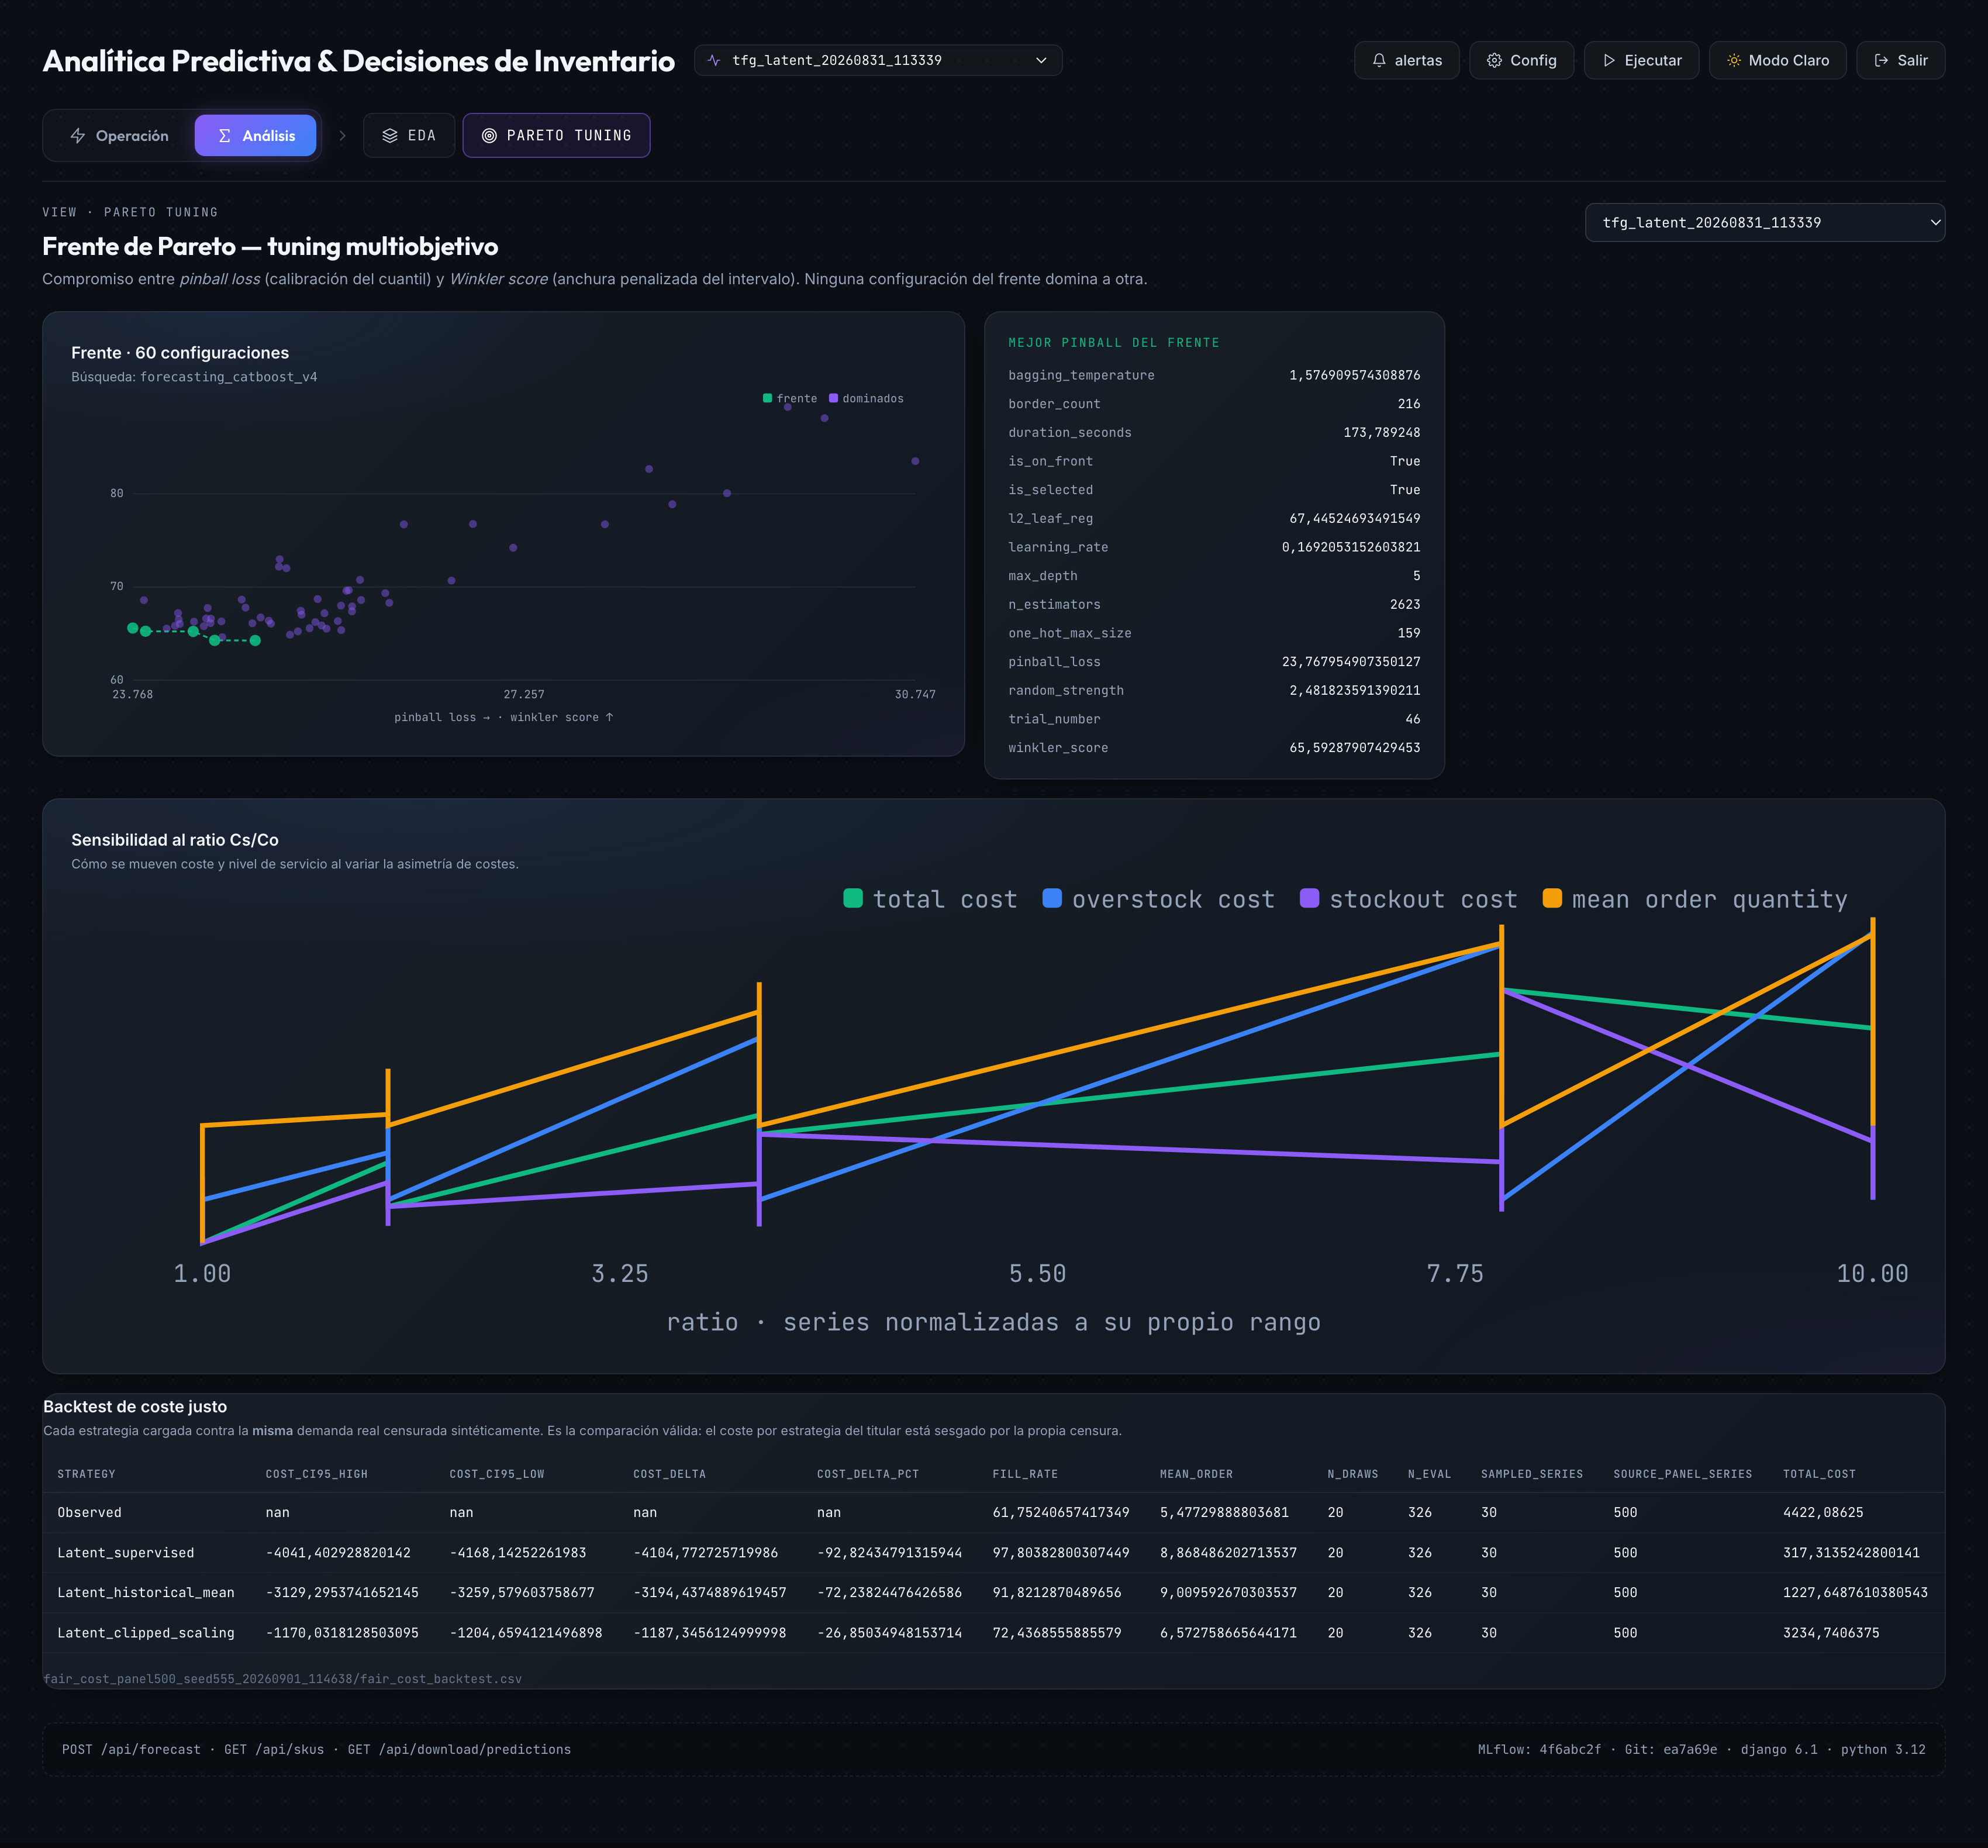
\includegraphics[width=\textwidth,height=0.82\textheight,keepaspectratio]{figures/dashboard/ui_pareto_tuning.png}
    \caption{Vista \textit{Pareto Tuning} del plano de Análisis, con los tres bloques que la componen. Arriba, el frente de la búsqueda multiobjetivo que nombra la propia tarjeta (\texttt{forecasting\_catboost\_v4}, 60 \textit{trials}): cada punto es una configuración situada por su \textit{pinball loss} y su \textit{Winkler score}, en verde las no dominadas y en violeta las dominadas, y a su derecha los hiperparámetros de la que minimiza el \textit{pinball} sobre el frente. En el centro, la sensibilidad al ratio $c_u/c_o$, con cada serie normalizada a su propio rango para que quepan en un eje común. Abajo, el \textit{backtest} de coste justo, que es la comparación que sí ordena las estrategias de reconstrucción (Sección~\ref{sec:resultados_gemelo}).}
    \label{fig:ui_pareto_tuning}
\end{figure}
